\documentclass[a4paper]{book}
\usepackage{makeidx}
\usepackage{natbib}
\usepackage{graphicx}
\usepackage{multicol}
\usepackage{float}
\usepackage{listings}
\usepackage{color}
\usepackage{ifthen}
\usepackage[table]{xcolor}
\usepackage{textcomp}
\usepackage{alltt}
\usepackage{ifpdf}
\ifpdf
\usepackage[pdftex,
            pagebackref=true,
            colorlinks=true,
            linkcolor=blue,
            unicode
           ]{hyperref}
\else
\usepackage[ps2pdf,
            pagebackref=true,
            colorlinks=true,
            linkcolor=blue,
            unicode
           ]{hyperref}
\usepackage{pspicture}
\fi
\usepackage[utf8]{inputenc}
\usepackage[brazil]{babel}
\usepackage{mathptmx}
\usepackage[scaled=.90]{helvet}
\usepackage{courier}
\usepackage{sectsty}
\usepackage[titles]{tocloft}
\usepackage{doxygen}
\lstset{language=C++,inputencoding=utf8,basicstyle=\footnotesize,breaklines=true,breakatwhitespace=true,tabsize=8,numbers=left }
\makeindex
\setcounter{tocdepth}{3}
\renewcommand{\footrulewidth}{0.4pt}
\renewcommand{\familydefault}{\sfdefault}
\hfuzz=15pt
\setlength{\emergencystretch}{15pt}
\hbadness=750
\tolerance=750
\begin{document}
\hypersetup{pageanchor=false,citecolor=blue}
\begin{titlepage}
\vspace*{7cm}
\begin{center}
{\Large \-Sistema de \-Projetos dos \-Alunos }\\
\vspace*{1cm}
{\large \-Gerado por Doxygen 1.7.5.1}\\
\vspace*{0.5cm}
{\small Segunda, 10 de Outubro de 2011 22:18:29}\\
\end{center}
\end{titlepage}
\clearemptydoublepage
\pagenumbering{roman}
\tableofcontents
\clearemptydoublepage
\pagenumbering{arabic}
\hypersetup{pageanchor=true,citecolor=blue}
\chapter{\-Sistema de \-Projetos de \-Alunos}
\label{index}\hypertarget{index}{}\-Esse sistema realiza os testes dos tipos basicos definidos no \-Sistema de \-Projeto de \-Alunos. \-Para cada tipo basico realiza-\/se um teste usando um argumento valido e um invalido. 
\chapter{Índice dos \-Componentes}
\section{\-Lista de componentes}
\-Lista de classes, estruturas, uniões e interfaces com uma breve descrição\-:\begin{DoxyCompactList}
\item\contentsline{section}{\hyperlink{class_cntr_int_fase}{\-Cntr\-Int\-Fase} \\*\-Classe que representa a controladora de interacao \-Usuario/\-Fase }{\pageref{class_cntr_int_fase}}{}
\item\contentsline{section}{\hyperlink{class_cntr_int_metrica}{\-Cntr\-Int\-Metrica} \\*\-Classe que representa a controladora de interacao \-Usuario/\-Metrica }{\pageref{class_cntr_int_metrica}}{}
\item\contentsline{section}{\hyperlink{class_cntr_int_modulo}{\-Cntr\-Int\-Modulo} \\*\-Classe que representa a controladora de interacao \-Usuario/\-Modulo }{\pageref{class_cntr_int_modulo}}{}
\item\contentsline{section}{\hyperlink{class_cntr_int_navegacao}{\-Cntr\-Int\-Navegacao} \\*\-Classe que representa a controladora de interacao \-Usuario/\-Navegacao }{\pageref{class_cntr_int_navegacao}}{}
\item\contentsline{section}{\hyperlink{class_cntr_int_projeto}{\-Cntr\-Int\-Projeto} \\*\-Classe que representa a controladora de interacao \-Usuario/\-Projeto }{\pageref{class_cntr_int_projeto}}{}
\item\contentsline{section}{\hyperlink{class_cntr_l_n_fase}{\-Cntr\-L\-N\-Fase} \\*\-Classe que representa a controladora de logica de negocio relacionada as fases }{\pageref{class_cntr_l_n_fase}}{}
\item\contentsline{section}{\hyperlink{class_cntr_l_n_metrica}{\-Cntr\-L\-N\-Metrica} \\*\-Classe que representa a controladora de logica de negocio relacionada as metricas }{\pageref{class_cntr_l_n_metrica}}{}
\item\contentsline{section}{\hyperlink{class_cntr_l_n_modulo}{\-Cntr\-L\-N\-Modulo} \\*\-Classe que representa a controladora de logica de negocio relacionada aos modulos }{\pageref{class_cntr_l_n_modulo}}{}
\item\contentsline{section}{\hyperlink{class_cntr_l_n_projeto}{\-Cntr\-L\-N\-Projeto} \\*\-Classe que representa a controladora de logica de negocio relacionada aos projetos }{\pageref{class_cntr_l_n_projeto}}{}
\item\contentsline{section}{\hyperlink{class_cntr_persistencia}{\-Cntr\-Persistencia} \\*\-Classe que representa a \-Controladora de \-Persistencia }{\pageref{class_cntr_persistencia}}{}
\item\contentsline{section}{\hyperlink{class_codigo___fase}{\-Codigo\-\_\-\-Fase} \\*\-Classe que representa o dominio \hyperlink{class_codigo___fase}{\-Codigo\-\_\-\-Fase} }{\pageref{class_codigo___fase}}{}
\item\contentsline{section}{\hyperlink{class_codigo___modulo}{\-Codigo\-\_\-\-Modulo} \\*\-Classe que representa o dominio \hyperlink{class_codigo___modulo}{\-Codigo\-\_\-\-Modulo} }{\pageref{class_codigo___modulo}}{}
\item\contentsline{section}{\hyperlink{class_codigo___projeto}{\-Codigo\-\_\-\-Projeto} \\*\-Classe que representa o dominio \hyperlink{class_codigo___projeto}{\-Codigo\-\_\-\-Projeto} }{\pageref{class_codigo___projeto}}{}
\item\contentsline{section}{\hyperlink{class_comando_atualizar_fase}{\-Comando\-Atualizar\-Fase} \\*\-Classe que simula servicos da classe \hyperlink{class_protocolo_persistencia}{\-Protocolo\-Persistencia} }{\pageref{class_comando_atualizar_fase}}{}
\item\contentsline{section}{\hyperlink{class_comando_atualizar_modulo}{\-Comando\-Atualizar\-Modulo} \\*\-Classe que simula servicos da classe \hyperlink{class_protocolo_persistencia}{\-Protocolo\-Persistencia} }{\pageref{class_comando_atualizar_modulo}}{}
\item\contentsline{section}{\hyperlink{class_comando_atualizar_projeto}{\-Comando\-Atualizar\-Projeto} \\*\-Classe que simula servicos da classe \hyperlink{class_protocolo_persistencia}{\-Protocolo\-Persistencia} }{\pageref{class_comando_atualizar_projeto}}{}
\item\contentsline{section}{\hyperlink{class_comando_b_d}{\-Comando\-B\-D} \\*\-Classe que representa os \-Comandos do \-Bando de \-Dados }{\pageref{class_comando_b_d}}{}
\item\contentsline{section}{\hyperlink{class_comando_cadastrar_fase}{\-Comando\-Cadastrar\-Fase} \\*\-Classe que simula servicos da classe \hyperlink{class_protocolo_persistencia}{\-Protocolo\-Persistencia} }{\pageref{class_comando_cadastrar_fase}}{}
\item\contentsline{section}{\hyperlink{class_comando_cadastrar_modulo}{\-Comando\-Cadastrar\-Modulo} \\*\-Classe que simula servicos da classe \hyperlink{class_protocolo_persistencia}{\-Protocolo\-Persistencia} }{\pageref{class_comando_cadastrar_modulo}}{}
\item\contentsline{section}{\hyperlink{class_comando_cadastrar_projeto}{\-Comando\-Cadastrar\-Projeto} \\*\-Classe que simula servicos da classe \hyperlink{class_protocolo_persistencia}{\-Protocolo\-Persistencia} }{\pageref{class_comando_cadastrar_projeto}}{}
\item\contentsline{section}{\hyperlink{class_comando_nota}{\-Comando\-Nota} \\*\-Classe \hyperlink{class_comando_nota}{\-Comando\-Nota} herda a classe comando\-B\-D e prove servicos para calcular as notas }{\pageref{class_comando_nota}}{}
\item\contentsline{section}{\hyperlink{class_comando_numero_linhas}{\-Comando\-Numero\-Linhas} \\*\-Classe \hyperlink{class_comando_numero_linhas}{\-Comando\-Numero\-Linhas} herda a classe comando\-B\-D e prove servicos para calcular o numero de linhas }{\pageref{class_comando_numero_linhas}}{}
\item\contentsline{section}{\hyperlink{class_comando_pesquisar_fase}{\-Comando\-Pesquisar\-Fase} \\*\-Classe que simula servicos da classe \hyperlink{class_protocolo_persistencia}{\-Protocolo\-Persistencia} }{\pageref{class_comando_pesquisar_fase}}{}
\item\contentsline{section}{\hyperlink{class_comando_pesquisar_modulo}{\-Comando\-Pesquisar\-Modulo} \\*\-Classe que simula servicos da classe \hyperlink{class_protocolo_persistencia}{\-Protocolo\-Persistencia} }{\pageref{class_comando_pesquisar_modulo}}{}
\item\contentsline{section}{\hyperlink{class_comando_pesquisar_projeto}{\-Comando\-Pesquisar\-Projeto} \\*\-Classe que simula servicos da classe \hyperlink{class_protocolo_persistencia}{\-Protocolo\-Persistencia} }{\pageref{class_comando_pesquisar_projeto}}{}
\item\contentsline{section}{\hyperlink{class_comando_produtividade_media}{\-Comando\-Produtividade\-Media} \\*\-Classe \hyperlink{class_comando_produtividade_media}{\-Comando\-Produtividade\-Media} herda a classe comando\-B\-D e prove servicos para calcular a produtividade media }{\pageref{class_comando_produtividade_media}}{}
\item\contentsline{section}{\hyperlink{class_comando_produtividade_modulo}{\-Comando\-Produtividade\-Modulo} \\*\-Classe \hyperlink{class_comando_produtividade_modulo}{\-Comando\-Produtividade\-Modulo} herda a classe comando\-B\-D e prove servicos para calcular a produtividade do modulo }{\pageref{class_comando_produtividade_modulo}}{}
\item\contentsline{section}{\hyperlink{class_comando_produtividade_projeto}{\-Comando\-Produtividade\-Projeto} \\*\-Classe \hyperlink{class_comando_produtividade_projeto}{\-Comando\-Produtividade\-Projeto} herda a classe comando\-B\-D e prove servicos para calcular a produtividade do projeto }{\pageref{class_comando_produtividade_projeto}}{}
\item\contentsline{section}{\hyperlink{class_comando_remover_fase}{\-Comando\-Remover\-Fase} \\*\-Classe que simula servicos da classe \hyperlink{class_protocolo_persistencia}{\-Protocolo\-Persistencia} }{\pageref{class_comando_remover_fase}}{}
\item\contentsline{section}{\hyperlink{class_comando_remover_modulo}{\-Comando\-Remover\-Modulo} \\*\-Classe que simula servicos da classe \hyperlink{class_protocolo_persistencia}{\-Protocolo\-Persistencia} }{\pageref{class_comando_remover_modulo}}{}
\item\contentsline{section}{\hyperlink{class_comando_remover_projeto}{\-Comando\-Remover\-Projeto} \\*\-Classe que simula servicos da classe \hyperlink{class_protocolo_persistencia}{\-Protocolo\-Persistencia} }{\pageref{class_comando_remover_projeto}}{}
\item\contentsline{section}{\hyperlink{class_comandos_modulo}{\-Comandos\-Modulo} \\*\-Classe \hyperlink{class_comandos_modulo}{\-Comandos\-Modulo} herda a classe \-Comandos\-B\-D e prove servicos pros comandos de \-Modulos }{\pageref{class_comandos_modulo}}{}
\item\contentsline{section}{\hyperlink{class_comandos_projeto}{\-Comandos\-Projeto} \\*\-Classe \hyperlink{class_comandos_projeto}{\-Comandos\-Projeto} herda a classe \-Comandos\-B\-D e prove servicos pros comandos de \-Projetos }{\pageref{class_comandos_projeto}}{}
\item\contentsline{section}{\hyperlink{class_comando_tamanho_medio}{\-Comando\-Tamanho\-Medio} \\*\-Classe \hyperlink{class_comando_tamanho_medio}{\-Comando\-Tamanho\-Medio} herda a classe comando\-B\-D e prove servicos para calcular o tamanho medio }{\pageref{class_comando_tamanho_medio}}{}
\item\contentsline{section}{\hyperlink{class_comando_tempo_gasto_modulo}{\-Comando\-Tempo\-Gasto\-Modulo} \\*\-Classe \hyperlink{class_comando_tempo_gasto_modulo}{\-Comando\-Tempo\-Gasto\-Modulo} herda a classe comando\-B\-D e prove servicos para calcular o tempo gasto no modulo }{\pageref{class_comando_tempo_gasto_modulo}}{}
\item\contentsline{section}{\hyperlink{class_comando_tempo_gasto_projeto}{\-Comando\-Tempo\-Gasto\-Projeto} \\*\-Classe \hyperlink{class_comando_tempo_gasto_projeto}{\-Comando\-Tempo\-Gasto\-Projeto} herda a classe comando\-B\-D e prove servicos para calcular o tempo gasto no projeto }{\pageref{class_comando_tempo_gasto_projeto}}{}
\item\contentsline{section}{\hyperlink{class_criar}{\-Criar} \\*\-Classe do padr�o de projeto \-Builder }{\pageref{class_criar}}{}
\item\contentsline{section}{\hyperlink{class_data___inicio}{\-Data\-\_\-\-Inicio} \\*\-Classe que representa o dominio \hyperlink{class_data___inicio}{\-Data\-\_\-\-Inicio} }{\pageref{class_data___inicio}}{}
\item\contentsline{section}{\hyperlink{class_data___termino}{\-Data\-\_\-\-Termino} \\*\-Classe que representa o dominio \hyperlink{class_data___termino}{\-Data\-\_\-\-Termino} }{\pageref{class_data___termino}}{}
\item\contentsline{section}{\hyperlink{class_e_erro_persistencia}{\-E\-Erro\-Persistencia} \\*\-Classe que representa o \-Erro \-Persistencia }{\pageref{class_e_erro_persistencia}}{}
\item\contentsline{section}{\hyperlink{class_elemento_resultado}{\-Elemento\-Resultado} \\*\-Classe que representa o \hyperlink{class_elemento_resultado}{\-Elemento\-Resultado} }{\pageref{class_elemento_resultado}}{}
\item\contentsline{section}{\hyperlink{class_fase}{\-Fase} \\*\-Classe que representa a entidade \hyperlink{class_fase}{\-Fase} }{\pageref{class_fase}}{}
\item\contentsline{section}{\hyperlink{class_matricula}{\-Matricula} \\*\-Classe que representa o dominio \hyperlink{class_matricula}{\-Matricula} }{\pageref{class_matricula}}{}
\item\contentsline{section}{\hyperlink{class_metrica}{\-Metrica} \\*\-Classe que representa a entidade \hyperlink{class_metrica}{\-Metrica} }{\pageref{class_metrica}}{}
\item\contentsline{section}{\hyperlink{class_modulo}{\-Modulo} \\*\-Classe que representa a entidade \hyperlink{class_modulo}{\-Modulo} }{\pageref{class_modulo}}{}
\item\contentsline{section}{\hyperlink{class_nome___arquivo}{\-Nome\-\_\-\-Arquivo} \\*\-Classe que representa o dominio \hyperlink{class_nome___arquivo}{\-Nome\-\_\-\-Arquivo} }{\pageref{class_nome___arquivo}}{}
\item\contentsline{section}{\hyperlink{class_nota}{\-Nota} \\*\-Classe que representa o dominio \hyperlink{class_nota}{\-Nota} }{\pageref{class_nota}}{}
\item\contentsline{section}{\hyperlink{class_projeto}{\-Projeto} \\*\-Classe que representa a entidade \hyperlink{class_projeto}{\-Projeto} }{\pageref{class_projeto}}{}
\item\contentsline{section}{\hyperlink{class_protocolo_fase}{\-Protocolo\-Fase} \\*\-Classe abstrata que faz a ligacao entre camada de interacao do usuario e logica de negocio }{\pageref{class_protocolo_fase}}{}
\item\contentsline{section}{\hyperlink{class_protocolo_int}{\-Protocolo\-Int} \\*\-Classe abstrata que e utilizada para a escolha das \-Controladoras de \-Interacao, atraves dos protocolos especificos }{\pageref{class_protocolo_int}}{}
\item\contentsline{section}{\hyperlink{class_protocolo_int_fase}{\-Protocolo\-Int\-Fase} \\*\-Classe abstrata que seleciona a \-Controladora de \hyperlink{class_fase}{\-Fase} }{\pageref{class_protocolo_int_fase}}{}
\item\contentsline{section}{\hyperlink{class_protocolo_int_metrica}{\-Protocolo\-Int\-Metrica} \\*\-Classe abstrata que seleciona a \-Controladora de \hyperlink{class_metrica}{\-Metrica} }{\pageref{class_protocolo_int_metrica}}{}
\item\contentsline{section}{\hyperlink{class_protocolo_int_modulo}{\-Protocolo\-Int\-Modulo} \\*\-Classe abstrata que seleciona a \-Controladora de \hyperlink{class_modulo}{\-Modulo} }{\pageref{class_protocolo_int_modulo}}{}
\item\contentsline{section}{\hyperlink{class_protocolo_int_projeto}{\-Protocolo\-Int\-Projeto} \\*\-Classe abstrata que seleciona a \-Controladora de \hyperlink{class_projeto}{\-Projeto} }{\pageref{class_protocolo_int_projeto}}{}
\item\contentsline{section}{\hyperlink{class_protocolo_metrica}{\-Protocolo\-Metrica} \\*\-Classe abstrata que faz a ligacao entre interacao do usuario e logica de negocio }{\pageref{class_protocolo_metrica}}{}
\item\contentsline{section}{\hyperlink{class_protocolo_modulo}{\-Protocolo\-Modulo} \\*\-Classe abstrata que faz a ligacao entre interacao do usuario e logica de negocio }{\pageref{class_protocolo_modulo}}{}
\item\contentsline{section}{\hyperlink{class_protocolo_persistencia}{\-Protocolo\-Persistencia} \\*\-Classe abstrata que representa o \-Protocolo de \-Persistencia }{\pageref{class_protocolo_persistencia}}{}
\item\contentsline{section}{\hyperlink{class_protocolo_projeto}{\-Protocolo\-Projeto} \\*\-Classe abstrata que faz a ligacao entre interacao do usuario e logica de negocio }{\pageref{class_protocolo_projeto}}{}
\item\contentsline{section}{\hyperlink{class_tamanho}{\-Tamanho} \\*\-Classe que representa o dominio \hyperlink{class_tamanho}{\-Tamanho} }{\pageref{class_tamanho}}{}
\item\contentsline{section}{\hyperlink{class_tempo}{\-Tempo} \\*\-Classe que representa o dominio \hyperlink{class_tempo}{\-Tempo} }{\pageref{class_tempo}}{}
\end{DoxyCompactList}

\chapter{\-Classes}
\hypertarget{class_codigo___fase}{
\section{\-Referência da \-Classe \-Codigo\-\_\-\-Fase}
\label{class_codigo___fase}\index{\-Codigo\-\_\-\-Fase@{\-Codigo\-\_\-\-Fase}}
}


\-Classe que representa o dominio \hyperlink{class_codigo___fase}{\-Codigo\-\_\-\-Fase}.  




{\ttfamily \#include $<$\-Dominios.\-h$>$}

\subsection*{\-Métodos \-Públicos}
\begin{DoxyCompactItemize}
\item 
\hypertarget{class_codigo___fase_a95e4aaa46eb3c9508216d9914f10de9b}{
{\bfseries \-Codigo\-\_\-\-Fase} (string)  throw (invalid\-\_\-argument)}
\label{class_codigo___fase_a95e4aaa46eb3c9508216d9914f10de9b}

\item 
void \hyperlink{class_codigo___fase_a30ddd9595c79d2ba10d25a857ae01704}{set\-Valor} (const string \&)  throw (invalid\-\_\-argument)
\begin{DoxyCompactList}\small\item\em \-Seta o valor de \-Codigo de \hyperlink{class_fase}{\-Fase}. \end{DoxyCompactList}\item 
string \hyperlink{class_codigo___fase_ad6211e7c092a64788fe6b007addd48d3}{get\-Valor} () const 
\begin{DoxyCompactList}\small\item\em \-Retorna o valor de \-Codigo de \hyperlink{class_fase}{\-Fase}. \end{DoxyCompactList}\end{DoxyCompactItemize}


\subsection{\-Descrição \-Detalhada}
\-Classe que representa o dominio \hyperlink{class_codigo___fase}{\-Codigo\-\_\-\-Fase}. 

\-Armazena os atributos de \-Codigo \-De \hyperlink{class_fase}{\-Fase} apos validacao\-: numero decimal composto por 1 digito 

\subsection{\-Métodos}
\hypertarget{class_codigo___fase_ad6211e7c092a64788fe6b007addd48d3}{
\index{\-Codigo\-\_\-\-Fase@{\-Codigo\-\_\-\-Fase}!get\-Valor@{get\-Valor}}
\index{get\-Valor@{get\-Valor}!Codigo_Fase@{\-Codigo\-\_\-\-Fase}}
\subsubsection[{get\-Valor}]{\setlength{\rightskip}{0pt plus 5cm}string \-Codigo\-\_\-\-Fase\-::get\-Valor (
\begin{DoxyParamCaption}
{}
\end{DoxyParamCaption}
) const\hspace{0.3cm}{\ttfamily  \mbox{[}inline\mbox{]}}}}
\label{class_codigo___fase_ad6211e7c092a64788fe6b007addd48d3}


\-Retorna o valor de \-Codigo de \hyperlink{class_fase}{\-Fase}. 

\begin{DoxyReturn}{\-Retorna}
valor 
\end{DoxyReturn}
\hypertarget{class_codigo___fase_a30ddd9595c79d2ba10d25a857ae01704}{
\index{\-Codigo\-\_\-\-Fase@{\-Codigo\-\_\-\-Fase}!set\-Valor@{set\-Valor}}
\index{set\-Valor@{set\-Valor}!Codigo_Fase@{\-Codigo\-\_\-\-Fase}}
\subsubsection[{set\-Valor}]{\setlength{\rightskip}{0pt plus 5cm}void \-Codigo\-\_\-\-Fase\-::set\-Valor (
\begin{DoxyParamCaption}
\item[{const string \&}]{valor}
\end{DoxyParamCaption}
)  throw (invalid\-\_\-argument)\hspace{0.3cm}{\ttfamily  \mbox{[}inline\mbox{]}}}}
\label{class_codigo___fase_a30ddd9595c79d2ba10d25a857ae01704}


\-Seta o valor de \-Codigo de \hyperlink{class_fase}{\-Fase}. 


\begin{DoxyParams}{\-Parâmetros}
{\em valor} & \\
\hline
\end{DoxyParams}


\-A documentação para esta classe foi gerada a partir do seguinte arquivo\-:\begin{DoxyCompactItemize}
\item 
header/\-Dominios.\-h\end{DoxyCompactItemize}

\hypertarget{class_codigo___modulo}{
\section{\-Referência à classe \-Codigo\-\_\-\-Modulo}
\label{class_codigo___modulo}\index{\-Codigo\-\_\-\-Modulo@{\-Codigo\-\_\-\-Modulo}}
}


\-Classe que representa o dominio \hyperlink{class_codigo___modulo}{\-Codigo\-\_\-\-Modulo}.  




{\ttfamily \#include $<$\-Dominios.\-h$>$}

\subsection*{\-Membros públicos}
\begin{DoxyCompactItemize}
\item 
\hypertarget{class_codigo___modulo_af02fd77a63061429f2951bc78741093e}{
{\bfseries \-Codigo\-\_\-\-Modulo} (string)  throw (invalid\-\_\-argument)}
\label{class_codigo___modulo_af02fd77a63061429f2951bc78741093e}

\item 
void \hyperlink{class_codigo___modulo_a974ed9c3733dcf75c362c53653e407e7}{set\-Valor} (const string \&)  throw (invalid\-\_\-argument)
\begin{DoxyCompactList}\small\item\em \-Seta o valor de \-Codigo de \hyperlink{class_modulo}{\-Modulo}. \end{DoxyCompactList}\item 
string \hyperlink{class_codigo___modulo_a87112e0fb26a7d32fe8cb06cc7d32746}{get\-Valor} () const 
\begin{DoxyCompactList}\small\item\em \-Retorna o valor de \-Codigo de \hyperlink{class_modulo}{\-Modulo}. \end{DoxyCompactList}\end{DoxyCompactItemize}


\subsection{\-Descrição detalhada}
\-Classe que representa o dominio \hyperlink{class_codigo___modulo}{\-Codigo\-\_\-\-Modulo}. 

\-Armazena os atributos de \-Codigo \-De \hyperlink{class_modulo}{\-Modulo} apos validacao\-: numero decimal composto por 5 digitos 

\subsection{\-Documentação dos métodos}
\hypertarget{class_codigo___modulo_a87112e0fb26a7d32fe8cb06cc7d32746}{
\index{\-Codigo\-\_\-\-Modulo@{\-Codigo\-\_\-\-Modulo}!get\-Valor@{get\-Valor}}
\index{get\-Valor@{get\-Valor}!Codigo_Modulo@{\-Codigo\-\_\-\-Modulo}}
\subsubsection[{get\-Valor}]{\setlength{\rightskip}{0pt plus 5cm}string \-Codigo\-\_\-\-Modulo\-::get\-Valor (
\begin{DoxyParamCaption}
{}
\end{DoxyParamCaption}
) const\hspace{0.3cm}{\ttfamily  \mbox{[}inline\mbox{]}}}}
\label{class_codigo___modulo_a87112e0fb26a7d32fe8cb06cc7d32746}


\-Retorna o valor de \-Codigo de \hyperlink{class_modulo}{\-Modulo}. 

\begin{DoxyReturn}{\-Retorna}
valor 
\end{DoxyReturn}
\hypertarget{class_codigo___modulo_a974ed9c3733dcf75c362c53653e407e7}{
\index{\-Codigo\-\_\-\-Modulo@{\-Codigo\-\_\-\-Modulo}!set\-Valor@{set\-Valor}}
\index{set\-Valor@{set\-Valor}!Codigo_Modulo@{\-Codigo\-\_\-\-Modulo}}
\subsubsection[{set\-Valor}]{\setlength{\rightskip}{0pt plus 5cm}void \-Codigo\-\_\-\-Modulo\-::set\-Valor (
\begin{DoxyParamCaption}
\item[{const string \&}]{valor}
\end{DoxyParamCaption}
)  throw (invalid\-\_\-argument)\hspace{0.3cm}{\ttfamily  \mbox{[}inline\mbox{]}}}}
\label{class_codigo___modulo_a974ed9c3733dcf75c362c53653e407e7}


\-Seta o valor de \-Codigo de \hyperlink{class_modulo}{\-Modulo}. 


\begin{DoxyParams}{\-Parâmetros}
{\em valor} & \\
\hline
\end{DoxyParams}


\-A documentação para esta classe foi gerada a partir do seguinte ficheiro\-:\begin{DoxyCompactItemize}
\item 
\-Dominios.\-h\end{DoxyCompactItemize}

\hypertarget{class_codigo___projeto}{
\section{\-Referência da \-Classe \-Codigo\-\_\-\-Projeto}
\label{class_codigo___projeto}\index{\-Codigo\-\_\-\-Projeto@{\-Codigo\-\_\-\-Projeto}}
}


\-Classe que representa o dominio \hyperlink{class_codigo___projeto}{\-Codigo\-\_\-\-Projeto}.  




{\ttfamily \#include $<$\-Dominios.\-h$>$}

\subsection*{\-Métodos \-Públicos}
\begin{DoxyCompactItemize}
\item 
\hypertarget{class_codigo___projeto_ac3aaa481366d852d0c654bac3f95bc97}{
{\bfseries \-Codigo\-\_\-\-Projeto} (string)  throw (invalid\-\_\-argument)}
\label{class_codigo___projeto_ac3aaa481366d852d0c654bac3f95bc97}

\item 
void \hyperlink{class_codigo___projeto_a8628c9fa45bb9be7c4b25ebfbe2c255c}{set\-Valor} (const string \&)  throw (invalid\-\_\-argument)
\begin{DoxyCompactList}\small\item\em \-Seta o valor de \-Codigo de \hyperlink{class_projeto}{\-Projeto}. \end{DoxyCompactList}\item 
string \hyperlink{class_codigo___projeto_ae2a6a32b20fcdd82dbafeef8cbec5bb2}{get\-Valor} () const 
\begin{DoxyCompactList}\small\item\em \-Retorna o valor de \-Codigo de \hyperlink{class_projeto}{\-Projeto}. \end{DoxyCompactList}\end{DoxyCompactItemize}


\subsection{\-Descrição \-Detalhada}
\-Classe que representa o dominio \hyperlink{class_codigo___projeto}{\-Codigo\-\_\-\-Projeto}. 

\-Armazena os atributos de \-Codigo \-De \hyperlink{class_projeto}{\-Projeto} apos validacao\-: numero decimal composto por 5 digitos 

\subsection{\-Métodos}
\hypertarget{class_codigo___projeto_ae2a6a32b20fcdd82dbafeef8cbec5bb2}{
\index{\-Codigo\-\_\-\-Projeto@{\-Codigo\-\_\-\-Projeto}!get\-Valor@{get\-Valor}}
\index{get\-Valor@{get\-Valor}!Codigo_Projeto@{\-Codigo\-\_\-\-Projeto}}
\subsubsection[{get\-Valor}]{\setlength{\rightskip}{0pt plus 5cm}string \-Codigo\-\_\-\-Projeto\-::get\-Valor (
\begin{DoxyParamCaption}
{}
\end{DoxyParamCaption}
) const\hspace{0.3cm}{\ttfamily  \mbox{[}inline\mbox{]}}}}
\label{class_codigo___projeto_ae2a6a32b20fcdd82dbafeef8cbec5bb2}


\-Retorna o valor de \-Codigo de \hyperlink{class_projeto}{\-Projeto}. 

\begin{DoxyReturn}{\-Retorna}
valor 
\end{DoxyReturn}
\hypertarget{class_codigo___projeto_a8628c9fa45bb9be7c4b25ebfbe2c255c}{
\index{\-Codigo\-\_\-\-Projeto@{\-Codigo\-\_\-\-Projeto}!set\-Valor@{set\-Valor}}
\index{set\-Valor@{set\-Valor}!Codigo_Projeto@{\-Codigo\-\_\-\-Projeto}}
\subsubsection[{set\-Valor}]{\setlength{\rightskip}{0pt plus 5cm}void \-Codigo\-\_\-\-Projeto\-::set\-Valor (
\begin{DoxyParamCaption}
\item[{const string \&}]{valor}
\end{DoxyParamCaption}
)  throw (invalid\-\_\-argument)\hspace{0.3cm}{\ttfamily  \mbox{[}inline\mbox{]}}}}
\label{class_codigo___projeto_a8628c9fa45bb9be7c4b25ebfbe2c255c}


\-Seta o valor de \-Codigo de \hyperlink{class_projeto}{\-Projeto}. 


\begin{DoxyParams}{\-Parâmetros}
{\em valor} & \\
\hline
\end{DoxyParams}


\-A documentação para esta classe foi gerada a partir do seguinte arquivo\-:\begin{DoxyCompactItemize}
\item 
header/\-Dominios.\-h\end{DoxyCompactItemize}

\hypertarget{class_data___inicio}{
\section{\-Referência à classe \-Data\-\_\-\-Inicio}
\label{class_data___inicio}\index{\-Data\-\_\-\-Inicio@{\-Data\-\_\-\-Inicio}}
}


\-Classe que representa o dominio \hyperlink{class_data___inicio}{\-Data\-\_\-\-Inicio}.  




{\ttfamily \#include $<$\-Dominios.\-h$>$}

\subsection*{\-Membros públicos}
\begin{DoxyCompactItemize}
\item 
\hypertarget{class_data___inicio_ad8c906741947b96d199ca5300704cd57}{
{\bfseries \-Data\-\_\-\-Inicio} (string)  throw (invalid\-\_\-argument)}
\label{class_data___inicio_ad8c906741947b96d199ca5300704cd57}

\item 
void \hyperlink{class_data___inicio_ad859eb0240b8e0eed36e3768855ed750}{set\-Valor} (const string \&)  throw (invalid\-\_\-argument)
\begin{DoxyCompactList}\small\item\em \-Seta o valor de \-Data de \-Inicio. \end{DoxyCompactList}\item 
string \hyperlink{class_data___inicio_ac2e2c96554bda3c8b2e1bacd0ce63682}{get\-Valor} () const 
\begin{DoxyCompactList}\small\item\em \-Retorna o valor de \-Data de \-Inicio. \end{DoxyCompactList}\end{DoxyCompactItemize}


\subsection{\-Descrição detalhada}
\-Classe que representa o dominio \hyperlink{class_data___inicio}{\-Data\-\_\-\-Inicio}. 

\-Armazena os atributos de \-Data \-Inicio apos validacao\-: \-D\-D/\-M\-M/\-A\-A\-A\-A 

\subsection{\-Documentação dos métodos}
\hypertarget{class_data___inicio_ac2e2c96554bda3c8b2e1bacd0ce63682}{
\index{\-Data\-\_\-\-Inicio@{\-Data\-\_\-\-Inicio}!get\-Valor@{get\-Valor}}
\index{get\-Valor@{get\-Valor}!Data_Inicio@{\-Data\-\_\-\-Inicio}}
\subsubsection[{get\-Valor}]{\setlength{\rightskip}{0pt plus 5cm}string \-Data\-\_\-\-Inicio\-::get\-Valor (
\begin{DoxyParamCaption}
{}
\end{DoxyParamCaption}
) const\hspace{0.3cm}{\ttfamily  \mbox{[}inline\mbox{]}}}}
\label{class_data___inicio_ac2e2c96554bda3c8b2e1bacd0ce63682}


\-Retorna o valor de \-Data de \-Inicio. 

\begin{DoxyReturn}{\-Retorna}
valor 
\end{DoxyReturn}
\hypertarget{class_data___inicio_ad859eb0240b8e0eed36e3768855ed750}{
\index{\-Data\-\_\-\-Inicio@{\-Data\-\_\-\-Inicio}!set\-Valor@{set\-Valor}}
\index{set\-Valor@{set\-Valor}!Data_Inicio@{\-Data\-\_\-\-Inicio}}
\subsubsection[{set\-Valor}]{\setlength{\rightskip}{0pt plus 5cm}void \-Data\-\_\-\-Inicio\-::set\-Valor (
\begin{DoxyParamCaption}
\item[{const string \&}]{valor}
\end{DoxyParamCaption}
)  throw (invalid\-\_\-argument)\hspace{0.3cm}{\ttfamily  \mbox{[}inline\mbox{]}}}}
\label{class_data___inicio_ad859eb0240b8e0eed36e3768855ed750}


\-Seta o valor de \-Data de \-Inicio. 


\begin{DoxyParams}{\-Parâmetros}
{\em valor} & \\
\hline
\end{DoxyParams}


\-A documentação para esta classe foi gerada a partir do seguinte ficheiro\-:\begin{DoxyCompactItemize}
\item 
\-Dominios.\-h\end{DoxyCompactItemize}

\hypertarget{class_data___termino}{
\section{\-Referência à classe \-Data\-\_\-\-Termino}
\label{class_data___termino}\index{\-Data\-\_\-\-Termino@{\-Data\-\_\-\-Termino}}
}


\-Classe que representa o dominio \hyperlink{class_data___termino}{\-Data\-\_\-\-Termino}.  




{\ttfamily \#include $<$\-Dominios.\-h$>$}

\subsection*{\-Membros públicos}
\begin{DoxyCompactItemize}
\item 
\hypertarget{class_data___termino_aba9f868e567e2d5c8c13197e77f1dc5c}{
{\bfseries \-Data\-\_\-\-Termino} (unsigned int)  throw (invalid\-\_\-argument)}
\label{class_data___termino_aba9f868e567e2d5c8c13197e77f1dc5c}

\item 
void \hyperlink{class_data___termino_a90fee567953e20e803b54da195132281}{set\-Valor} (const unsigned int \&)  throw (invalid\-\_\-argument)
\begin{DoxyCompactList}\small\item\em \-Seta o valor de \-Data de \-Termino. \end{DoxyCompactList}\item 
unsigned int \hyperlink{class_data___termino_ad5265c6ec1c563ed89f4fc9a6588ac8b}{get\-Valor} () const 
\begin{DoxyCompactList}\small\item\em \-Retorna o valor de \-Data de \-Termino. \end{DoxyCompactList}\end{DoxyCompactItemize}


\subsection{\-Descrição detalhada}
\-Classe que representa o dominio \hyperlink{class_data___termino}{\-Data\-\_\-\-Termino}. 

\-Armazena os atributos de \-Data \-Termino apos validacao\-: \-D\-D/\-M\-M/\-A\-A\-A\-A 

\subsection{\-Documentação dos métodos}
\hypertarget{class_data___termino_ad5265c6ec1c563ed89f4fc9a6588ac8b}{
\index{\-Data\-\_\-\-Termino@{\-Data\-\_\-\-Termino}!get\-Valor@{get\-Valor}}
\index{get\-Valor@{get\-Valor}!Data_Termino@{\-Data\-\_\-\-Termino}}
\subsubsection[{get\-Valor}]{\setlength{\rightskip}{0pt plus 5cm}unsigned int \-Data\-\_\-\-Termino\-::get\-Valor (
\begin{DoxyParamCaption}
{}
\end{DoxyParamCaption}
) const\hspace{0.3cm}{\ttfamily  \mbox{[}inline\mbox{]}}}}
\label{class_data___termino_ad5265c6ec1c563ed89f4fc9a6588ac8b}


\-Retorna o valor de \-Data de \-Termino. 

\begin{DoxyReturn}{\-Retorna}
valor 
\end{DoxyReturn}
\hypertarget{class_data___termino_a90fee567953e20e803b54da195132281}{
\index{\-Data\-\_\-\-Termino@{\-Data\-\_\-\-Termino}!set\-Valor@{set\-Valor}}
\index{set\-Valor@{set\-Valor}!Data_Termino@{\-Data\-\_\-\-Termino}}
\subsubsection[{set\-Valor}]{\setlength{\rightskip}{0pt plus 5cm}void \-Data\-\_\-\-Termino\-::set\-Valor (
\begin{DoxyParamCaption}
\item[{const unsigned int \&}]{valor}
\end{DoxyParamCaption}
)  throw (invalid\-\_\-argument)\hspace{0.3cm}{\ttfamily  \mbox{[}inline\mbox{]}}}}
\label{class_data___termino_a90fee567953e20e803b54da195132281}


\-Seta o valor de \-Data de \-Termino. 


\begin{DoxyParams}{\-Parâmetros}
{\em valor} & \\
\hline
\end{DoxyParams}


\-A documentação para esta classe foi gerada a partir do seguinte ficheiro\-:\begin{DoxyCompactItemize}
\item 
\-Dominios.\-h\end{DoxyCompactItemize}

\hypertarget{class_fase}{
\section{\-Referência da \-Classe \-Fase}
\label{class_fase}\index{\-Fase@{\-Fase}}
}


\-Classe que representa a entidade \hyperlink{class_fase}{\-Fase}.  




{\ttfamily \#include $<$\-Entidades.\-h$>$}

\subsection*{\-Métodos \-Públicos}
\begin{DoxyCompactItemize}
\item 
\hypertarget{class_fase_a01205110dcfe61f938e5cbbda81f458f}{
{\bfseries \-Fase} (\hyperlink{class_codigo___fase}{\-Codigo\-\_\-\-Fase}, \hyperlink{class_tempo}{\-Tempo}, \hyperlink{class_tempo}{\-Tempo})}
\label{class_fase_a01205110dcfe61f938e5cbbda81f458f}

\item 
\hyperlink{class_codigo___fase}{\-Codigo\-\_\-\-Fase} \hyperlink{class_fase_a602d9dcd3d2cc62a38815cc92bb2544e}{get\-Codigo\-\_\-\-Fase} () const 
\begin{DoxyCompactList}\small\item\em \-Retorna o valor de \-Codigo de \hyperlink{class_fase}{\-Fase}. \end{DoxyCompactList}\item 
void \hyperlink{class_fase_a8558fc7a14dedece24cb05ef45a468ed}{set\-Codigo\-\_\-\-Fase} (const \hyperlink{class_codigo___fase}{\-Codigo\-\_\-\-Fase} \&)
\begin{DoxyCompactList}\small\item\em \-Seta o valor de \-Codigo de \hyperlink{class_fase}{\-Fase}. \end{DoxyCompactList}\item 
\hyperlink{class_tempo}{\-Tempo} \hyperlink{class_fase_a2745e6795ee74841ab2568bd6634677f}{get\-Tempo\-\_\-\-Estimado} () const 
\begin{DoxyCompactList}\small\item\em \-Retorna o valor de \hyperlink{class_tempo}{\-Tempo} \-Estimado. \end{DoxyCompactList}\item 
void \hyperlink{class_fase_a03725dee42c6222b00278c1e6b335ab7}{set\-Tempo\-\_\-\-Estimado} (const \hyperlink{class_tempo}{\-Tempo} \&)
\begin{DoxyCompactList}\small\item\em \-Seta o valor de \hyperlink{class_tempo}{\-Tempo} \-Estimado. \end{DoxyCompactList}\item 
\hyperlink{class_tempo}{\-Tempo} \hyperlink{class_fase_a19537f118a435b148749fdd965e33e7a}{get\-Tempo\-\_\-\-Efetivo} () const 
\begin{DoxyCompactList}\small\item\em \-Retorna o valor de \hyperlink{class_tempo}{\-Tempo} \-Efetivo. \end{DoxyCompactList}\item 
void \hyperlink{class_fase_ad804992aa80bdb68e6414ab2c16f2e70}{set\-Tempo\-\_\-\-Efetivo} (const \hyperlink{class_tempo}{\-Tempo} \&)
\begin{DoxyCompactList}\small\item\em \-Seta o valor de \hyperlink{class_tempo}{\-Tempo} \-Efetivo. \end{DoxyCompactList}\end{DoxyCompactItemize}


\subsection{\-Descrição \-Detalhada}
\-Classe que representa a entidade \hyperlink{class_fase}{\-Fase}. 

\-Contem os atributos que sao instancias das classes \hyperlink{class_codigo___fase}{\-Codigo\-\_\-\-Fase} e \hyperlink{class_tempo}{\-Tempo} 

\subsection{\-Métodos}
\hypertarget{class_fase_a602d9dcd3d2cc62a38815cc92bb2544e}{
\index{\-Fase@{\-Fase}!get\-Codigo\-\_\-\-Fase@{get\-Codigo\-\_\-\-Fase}}
\index{get\-Codigo\-\_\-\-Fase@{get\-Codigo\-\_\-\-Fase}!Fase@{\-Fase}}
\subsubsection[{get\-Codigo\-\_\-\-Fase}]{\setlength{\rightskip}{0pt plus 5cm}{\bf \-Codigo\-\_\-\-Fase} \-Fase\-::get\-Codigo\-\_\-\-Fase (
\begin{DoxyParamCaption}
{}
\end{DoxyParamCaption}
) const\hspace{0.3cm}{\ttfamily  \mbox{[}inline\mbox{]}}}}
\label{class_fase_a602d9dcd3d2cc62a38815cc92bb2544e}


\-Retorna o valor de \-Codigo de \hyperlink{class_fase}{\-Fase}. 

\begin{DoxyReturn}{\-Retorna}
valor 
\end{DoxyReturn}
\hypertarget{class_fase_a19537f118a435b148749fdd965e33e7a}{
\index{\-Fase@{\-Fase}!get\-Tempo\-\_\-\-Efetivo@{get\-Tempo\-\_\-\-Efetivo}}
\index{get\-Tempo\-\_\-\-Efetivo@{get\-Tempo\-\_\-\-Efetivo}!Fase@{\-Fase}}
\subsubsection[{get\-Tempo\-\_\-\-Efetivo}]{\setlength{\rightskip}{0pt plus 5cm}{\bf \-Tempo} \-Fase\-::get\-Tempo\-\_\-\-Efetivo (
\begin{DoxyParamCaption}
{}
\end{DoxyParamCaption}
) const\hspace{0.3cm}{\ttfamily  \mbox{[}inline\mbox{]}}}}
\label{class_fase_a19537f118a435b148749fdd965e33e7a}


\-Retorna o valor de \hyperlink{class_tempo}{\-Tempo} \-Efetivo. 

\begin{DoxyReturn}{\-Retorna}
valor 
\end{DoxyReturn}
\hypertarget{class_fase_a2745e6795ee74841ab2568bd6634677f}{
\index{\-Fase@{\-Fase}!get\-Tempo\-\_\-\-Estimado@{get\-Tempo\-\_\-\-Estimado}}
\index{get\-Tempo\-\_\-\-Estimado@{get\-Tempo\-\_\-\-Estimado}!Fase@{\-Fase}}
\subsubsection[{get\-Tempo\-\_\-\-Estimado}]{\setlength{\rightskip}{0pt plus 5cm}{\bf \-Tempo} \-Fase\-::get\-Tempo\-\_\-\-Estimado (
\begin{DoxyParamCaption}
{}
\end{DoxyParamCaption}
) const\hspace{0.3cm}{\ttfamily  \mbox{[}inline\mbox{]}}}}
\label{class_fase_a2745e6795ee74841ab2568bd6634677f}


\-Retorna o valor de \hyperlink{class_tempo}{\-Tempo} \-Estimado. 

\begin{DoxyReturn}{\-Retorna}
valor 
\end{DoxyReturn}
\hypertarget{class_fase_a8558fc7a14dedece24cb05ef45a468ed}{
\index{\-Fase@{\-Fase}!set\-Codigo\-\_\-\-Fase@{set\-Codigo\-\_\-\-Fase}}
\index{set\-Codigo\-\_\-\-Fase@{set\-Codigo\-\_\-\-Fase}!Fase@{\-Fase}}
\subsubsection[{set\-Codigo\-\_\-\-Fase}]{\setlength{\rightskip}{0pt plus 5cm}void \-Fase\-::set\-Codigo\-\_\-\-Fase (
\begin{DoxyParamCaption}
\item[{const {\bf \-Codigo\-\_\-\-Fase} \&}]{}
\end{DoxyParamCaption}
)}}
\label{class_fase_a8558fc7a14dedece24cb05ef45a468ed}


\-Seta o valor de \-Codigo de \hyperlink{class_fase}{\-Fase}. 


\begin{DoxyParams}{\-Parâmetros}
{\em valor} & \\
\hline
\end{DoxyParams}
\hypertarget{class_fase_ad804992aa80bdb68e6414ab2c16f2e70}{
\index{\-Fase@{\-Fase}!set\-Tempo\-\_\-\-Efetivo@{set\-Tempo\-\_\-\-Efetivo}}
\index{set\-Tempo\-\_\-\-Efetivo@{set\-Tempo\-\_\-\-Efetivo}!Fase@{\-Fase}}
\subsubsection[{set\-Tempo\-\_\-\-Efetivo}]{\setlength{\rightskip}{0pt plus 5cm}void \-Fase\-::set\-Tempo\-\_\-\-Efetivo (
\begin{DoxyParamCaption}
\item[{const {\bf \-Tempo} \&}]{}
\end{DoxyParamCaption}
)}}
\label{class_fase_ad804992aa80bdb68e6414ab2c16f2e70}


\-Seta o valor de \hyperlink{class_tempo}{\-Tempo} \-Efetivo. 


\begin{DoxyParams}{\-Parâmetros}
{\em valor} & \\
\hline
\end{DoxyParams}
\hypertarget{class_fase_a03725dee42c6222b00278c1e6b335ab7}{
\index{\-Fase@{\-Fase}!set\-Tempo\-\_\-\-Estimado@{set\-Tempo\-\_\-\-Estimado}}
\index{set\-Tempo\-\_\-\-Estimado@{set\-Tempo\-\_\-\-Estimado}!Fase@{\-Fase}}
\subsubsection[{set\-Tempo\-\_\-\-Estimado}]{\setlength{\rightskip}{0pt plus 5cm}void \-Fase\-::set\-Tempo\-\_\-\-Estimado (
\begin{DoxyParamCaption}
\item[{const {\bf \-Tempo} \&}]{}
\end{DoxyParamCaption}
)}}
\label{class_fase_a03725dee42c6222b00278c1e6b335ab7}


\-Seta o valor de \hyperlink{class_tempo}{\-Tempo} \-Estimado. 


\begin{DoxyParams}{\-Parâmetros}
{\em valor} & \\
\hline
\end{DoxyParams}


\-A documentação para esta classe foi gerada a partir do seguinte arquivo\-:\begin{DoxyCompactItemize}
\item 
header/\-Entidades.\-h\end{DoxyCompactItemize}

\hypertarget{class_matricula}{
\section{\-Referência à classe \-Matricula}
\label{class_matricula}\index{\-Matricula@{\-Matricula}}
}


\-Classe que representa o dominio \hyperlink{class_matricula}{\-Matricula}.  




{\ttfamily \#include $<$\-Dominios.\-h$>$}

\subsection*{\-Membros públicos}
\begin{DoxyCompactItemize}
\item 
\hypertarget{class_matricula_ad0e207a892bf8ae631a9374d9998996c}{
{\bfseries \-Matricula} (string)  throw (invalid\-\_\-argument)}
\label{class_matricula_ad0e207a892bf8ae631a9374d9998996c}

\item 
void \hyperlink{class_matricula_a0b767fcc96039728967640a19683aecd}{set\-Valor} (const string \&)  throw (invalid\-\_\-argument)
\begin{DoxyCompactList}\small\item\em \-Seta o valor de \hyperlink{class_matricula}{\-Matricula}. \end{DoxyCompactList}\item 
string \hyperlink{class_matricula_a5be68782efe39d296add81af1f4a8cc2}{get\-Valor} () const 
\begin{DoxyCompactList}\small\item\em \-Retorna o valor de \hyperlink{class_matricula}{\-Matricula}. \end{DoxyCompactList}\end{DoxyCompactItemize}


\subsection{\-Descrição detalhada}
\-Classe que representa o dominio \hyperlink{class_matricula}{\-Matricula}. 

\-Armazena os atributos de \hyperlink{class_matricula}{\-Matricula} apos validacao\-: numero decimal composto por 5 digitos 

\subsection{\-Documentação dos métodos}
\hypertarget{class_matricula_a5be68782efe39d296add81af1f4a8cc2}{
\index{\-Matricula@{\-Matricula}!get\-Valor@{get\-Valor}}
\index{get\-Valor@{get\-Valor}!Matricula@{\-Matricula}}
\subsubsection[{get\-Valor}]{\setlength{\rightskip}{0pt plus 5cm}string \-Matricula\-::get\-Valor (
\begin{DoxyParamCaption}
{}
\end{DoxyParamCaption}
) const\hspace{0.3cm}{\ttfamily  \mbox{[}inline\mbox{]}}}}
\label{class_matricula_a5be68782efe39d296add81af1f4a8cc2}


\-Retorna o valor de \hyperlink{class_matricula}{\-Matricula}. 

\begin{DoxyReturn}{\-Retorna}
valor 
\end{DoxyReturn}
\hypertarget{class_matricula_a0b767fcc96039728967640a19683aecd}{
\index{\-Matricula@{\-Matricula}!set\-Valor@{set\-Valor}}
\index{set\-Valor@{set\-Valor}!Matricula@{\-Matricula}}
\subsubsection[{set\-Valor}]{\setlength{\rightskip}{0pt plus 5cm}void \-Matricula\-::set\-Valor (
\begin{DoxyParamCaption}
\item[{const string \&}]{valor}
\end{DoxyParamCaption}
)  throw (invalid\-\_\-argument)\hspace{0.3cm}{\ttfamily  \mbox{[}inline\mbox{]}}}}
\label{class_matricula_a0b767fcc96039728967640a19683aecd}


\-Seta o valor de \hyperlink{class_matricula}{\-Matricula}. 


\begin{DoxyParams}{\-Parâmetros}
{\em valor} & \\
\hline
\end{DoxyParams}


\-A documentação para esta classe foi gerada a partir do seguinte ficheiro\-:\begin{DoxyCompactItemize}
\item 
\-Dominios.\-h\end{DoxyCompactItemize}

\hypertarget{class_modulo}{
\section{\-Referência da \-Classe \-Modulo}
\label{class_modulo}\index{\-Modulo@{\-Modulo}}
}


\-Classe que representa a entidade \hyperlink{class_modulo}{\-Modulo}.  




{\ttfamily \#include $<$\-Entidades.\-h$>$}

\subsection*{\-Métodos \-Públicos}
\begin{DoxyCompactItemize}
\item 
\hypertarget{class_modulo_ad4dc51b22b8bd726070b683fce87fa52}{
{\bfseries \-Modulo} (\hyperlink{class_codigo___modulo}{\-Codigo\-\_\-\-Modulo}, \hyperlink{class_nome___arquivo}{\-Nome\-\_\-\-Arquivo}, \hyperlink{class_tamanho}{\-Tamanho})}
\label{class_modulo_ad4dc51b22b8bd726070b683fce87fa52}

\item 
\hyperlink{class_codigo___modulo}{\-Codigo\-\_\-\-Modulo} \hyperlink{class_modulo_a966939d6761114d5030ca10c816302ac}{get\-Codigo\-\_\-\-Modulo} () const 
\begin{DoxyCompactList}\small\item\em \-Retorna o valor de \-Codigo de \hyperlink{class_modulo}{\-Modulo}. \end{DoxyCompactList}\item 
void \hyperlink{class_modulo_a8b41e4725c45aa47b5454008f517c392}{set\-Codigo\-\_\-\-Modulo} (const \hyperlink{class_codigo___modulo}{\-Codigo\-\_\-\-Modulo} \&)
\begin{DoxyCompactList}\small\item\em \-Seta o valor de \-Codigo de \hyperlink{class_modulo}{\-Modulo}. \end{DoxyCompactList}\item 
\hyperlink{class_nome___arquivo}{\-Nome\-\_\-\-Arquivo} \hyperlink{class_modulo_af4662253c0b78f248b02e3925a5d102c}{get\-Nome\-\_\-\-Arquivo} () const 
\begin{DoxyCompactList}\small\item\em \-Retorna o valor de \-Nome de \-Arquivo. \end{DoxyCompactList}\item 
void \hyperlink{class_modulo_a52d8354c7eb434f05ea76fbbcf715f9b}{set\-Nome\-\_\-\-Arquivo} (const \hyperlink{class_nome___arquivo}{\-Nome\-\_\-\-Arquivo} \&)
\begin{DoxyCompactList}\small\item\em \-Seta o valor de \-Nome de \-Arquivo. \end{DoxyCompactList}\item 
\hyperlink{class_tamanho}{\-Tamanho} \hyperlink{class_modulo_a64213272a845de661228d9117560d405}{get\-Tamanho} () const 
\begin{DoxyCompactList}\small\item\em \-Retorna o valor de \hyperlink{class_tamanho}{\-Tamanho}. \end{DoxyCompactList}\item 
void \hyperlink{class_modulo_ac39f3f24b46921700cd9231b2b67ddd9}{set\-Tamanho} (const \hyperlink{class_tamanho}{\-Tamanho} \&)
\begin{DoxyCompactList}\small\item\em \-Seta o valor de \hyperlink{class_tamanho}{\-Tamanho}. \end{DoxyCompactList}\end{DoxyCompactItemize}


\subsection{\-Descrição \-Detalhada}
\-Classe que representa a entidade \hyperlink{class_modulo}{\-Modulo}. 

\-Contem os atributos que sao instancias das classes \hyperlink{class_codigo___modulo}{\-Codigo\-\_\-\-Modulo}, \hyperlink{class_nome___arquivo}{\-Nome\-\_\-\-Arquivo} e \hyperlink{class_tamanho}{\-Tamanho} 

\subsection{\-Métodos}
\hypertarget{class_modulo_a966939d6761114d5030ca10c816302ac}{
\index{\-Modulo@{\-Modulo}!get\-Codigo\-\_\-\-Modulo@{get\-Codigo\-\_\-\-Modulo}}
\index{get\-Codigo\-\_\-\-Modulo@{get\-Codigo\-\_\-\-Modulo}!Modulo@{\-Modulo}}
\subsubsection[{get\-Codigo\-\_\-\-Modulo}]{\setlength{\rightskip}{0pt plus 5cm}{\bf \-Codigo\-\_\-\-Modulo} \-Modulo\-::get\-Codigo\-\_\-\-Modulo (
\begin{DoxyParamCaption}
{}
\end{DoxyParamCaption}
) const\hspace{0.3cm}{\ttfamily  \mbox{[}inline\mbox{]}}}}
\label{class_modulo_a966939d6761114d5030ca10c816302ac}


\-Retorna o valor de \-Codigo de \hyperlink{class_modulo}{\-Modulo}. 

\begin{DoxyReturn}{\-Retorna}
valor 
\end{DoxyReturn}
\hypertarget{class_modulo_af4662253c0b78f248b02e3925a5d102c}{
\index{\-Modulo@{\-Modulo}!get\-Nome\-\_\-\-Arquivo@{get\-Nome\-\_\-\-Arquivo}}
\index{get\-Nome\-\_\-\-Arquivo@{get\-Nome\-\_\-\-Arquivo}!Modulo@{\-Modulo}}
\subsubsection[{get\-Nome\-\_\-\-Arquivo}]{\setlength{\rightskip}{0pt plus 5cm}{\bf \-Nome\-\_\-\-Arquivo} \-Modulo\-::get\-Nome\-\_\-\-Arquivo (
\begin{DoxyParamCaption}
{}
\end{DoxyParamCaption}
) const\hspace{0.3cm}{\ttfamily  \mbox{[}inline\mbox{]}}}}
\label{class_modulo_af4662253c0b78f248b02e3925a5d102c}


\-Retorna o valor de \-Nome de \-Arquivo. 

\begin{DoxyReturn}{\-Retorna}
valor 
\end{DoxyReturn}
\hypertarget{class_modulo_a64213272a845de661228d9117560d405}{
\index{\-Modulo@{\-Modulo}!get\-Tamanho@{get\-Tamanho}}
\index{get\-Tamanho@{get\-Tamanho}!Modulo@{\-Modulo}}
\subsubsection[{get\-Tamanho}]{\setlength{\rightskip}{0pt plus 5cm}{\bf \-Tamanho} \-Modulo\-::get\-Tamanho (
\begin{DoxyParamCaption}
{}
\end{DoxyParamCaption}
) const\hspace{0.3cm}{\ttfamily  \mbox{[}inline\mbox{]}}}}
\label{class_modulo_a64213272a845de661228d9117560d405}


\-Retorna o valor de \hyperlink{class_tamanho}{\-Tamanho}. 

\begin{DoxyReturn}{\-Retorna}
valor 
\end{DoxyReturn}
\hypertarget{class_modulo_a8b41e4725c45aa47b5454008f517c392}{
\index{\-Modulo@{\-Modulo}!set\-Codigo\-\_\-\-Modulo@{set\-Codigo\-\_\-\-Modulo}}
\index{set\-Codigo\-\_\-\-Modulo@{set\-Codigo\-\_\-\-Modulo}!Modulo@{\-Modulo}}
\subsubsection[{set\-Codigo\-\_\-\-Modulo}]{\setlength{\rightskip}{0pt plus 5cm}void \-Modulo\-::set\-Codigo\-\_\-\-Modulo (
\begin{DoxyParamCaption}
\item[{const {\bf \-Codigo\-\_\-\-Modulo} \&}]{}
\end{DoxyParamCaption}
)}}
\label{class_modulo_a8b41e4725c45aa47b5454008f517c392}


\-Seta o valor de \-Codigo de \hyperlink{class_modulo}{\-Modulo}. 


\begin{DoxyParams}{\-Parâmetros}
{\em valor} & \\
\hline
\end{DoxyParams}
\hypertarget{class_modulo_a52d8354c7eb434f05ea76fbbcf715f9b}{
\index{\-Modulo@{\-Modulo}!set\-Nome\-\_\-\-Arquivo@{set\-Nome\-\_\-\-Arquivo}}
\index{set\-Nome\-\_\-\-Arquivo@{set\-Nome\-\_\-\-Arquivo}!Modulo@{\-Modulo}}
\subsubsection[{set\-Nome\-\_\-\-Arquivo}]{\setlength{\rightskip}{0pt plus 5cm}void \-Modulo\-::set\-Nome\-\_\-\-Arquivo (
\begin{DoxyParamCaption}
\item[{const {\bf \-Nome\-\_\-\-Arquivo} \&}]{}
\end{DoxyParamCaption}
)}}
\label{class_modulo_a52d8354c7eb434f05ea76fbbcf715f9b}


\-Seta o valor de \-Nome de \-Arquivo. 


\begin{DoxyParams}{\-Parâmetros}
{\em valor} & \\
\hline
\end{DoxyParams}
\hypertarget{class_modulo_ac39f3f24b46921700cd9231b2b67ddd9}{
\index{\-Modulo@{\-Modulo}!set\-Tamanho@{set\-Tamanho}}
\index{set\-Tamanho@{set\-Tamanho}!Modulo@{\-Modulo}}
\subsubsection[{set\-Tamanho}]{\setlength{\rightskip}{0pt plus 5cm}void \-Modulo\-::set\-Tamanho (
\begin{DoxyParamCaption}
\item[{const {\bf \-Tamanho} \&}]{}
\end{DoxyParamCaption}
)}}
\label{class_modulo_ac39f3f24b46921700cd9231b2b67ddd9}


\-Seta o valor de \hyperlink{class_tamanho}{\-Tamanho}. 


\begin{DoxyParams}{\-Parâmetros}
{\em valor} & \\
\hline
\end{DoxyParams}


\-A documentação para esta classe foi gerada a partir do seguinte arquivo\-:\begin{DoxyCompactItemize}
\item 
header/\-Entidades.\-h\end{DoxyCompactItemize}

\hypertarget{class_nome___arquivo}{
\section{\-Referência da \-Classe \-Nome\-\_\-\-Arquivo}
\label{class_nome___arquivo}\index{\-Nome\-\_\-\-Arquivo@{\-Nome\-\_\-\-Arquivo}}
}


\-Classe que representa o dominio \hyperlink{class_nome___arquivo}{\-Nome\-\_\-\-Arquivo}.  




{\ttfamily \#include $<$\-Dominios.\-h$>$}

\subsection*{\-Métodos \-Públicos}
\begin{DoxyCompactItemize}
\item 
\hypertarget{class_nome___arquivo_a94184c5ebb4b36edd83f95258fa1a816}{
{\bfseries \-Nome\-\_\-\-Arquivo} (string)  throw (invalid\-\_\-argument)}
\label{class_nome___arquivo_a94184c5ebb4b36edd83f95258fa1a816}

\item 
void \hyperlink{class_nome___arquivo_a93ccb1b3f4c3458075dfa949a8d86201}{set\-Valor} (const string \&)  throw (invalid\-\_\-argument)
\begin{DoxyCompactList}\small\item\em \-Seta o valor de \-Nome do \-Arquivo. \end{DoxyCompactList}\item 
string \hyperlink{class_nome___arquivo_a265da0a7dc6a42300a7955bba9f6fcfa}{get\-Valor} () const 
\begin{DoxyCompactList}\small\item\em \-Retorna o valor de \-Nome do \-Arquivo. \end{DoxyCompactList}\end{DoxyCompactItemize}


\subsection{\-Descrição \-Detalhada}
\-Classe que representa o dominio \hyperlink{class_nome___arquivo}{\-Nome\-\_\-\-Arquivo}. 

\-Armazena os atributos de \-Nome de \-Arquivo apos validacao\-: 10 caracteres quaisquer 

\subsection{\-Métodos}
\hypertarget{class_nome___arquivo_a265da0a7dc6a42300a7955bba9f6fcfa}{
\index{\-Nome\-\_\-\-Arquivo@{\-Nome\-\_\-\-Arquivo}!get\-Valor@{get\-Valor}}
\index{get\-Valor@{get\-Valor}!Nome_Arquivo@{\-Nome\-\_\-\-Arquivo}}
\subsubsection[{get\-Valor}]{\setlength{\rightskip}{0pt plus 5cm}string \-Nome\-\_\-\-Arquivo\-::get\-Valor (
\begin{DoxyParamCaption}
{}
\end{DoxyParamCaption}
) const\hspace{0.3cm}{\ttfamily  \mbox{[}inline\mbox{]}}}}
\label{class_nome___arquivo_a265da0a7dc6a42300a7955bba9f6fcfa}


\-Retorna o valor de \-Nome do \-Arquivo. 

\begin{DoxyReturn}{\-Retorna}
valor 
\end{DoxyReturn}
\hypertarget{class_nome___arquivo_a93ccb1b3f4c3458075dfa949a8d86201}{
\index{\-Nome\-\_\-\-Arquivo@{\-Nome\-\_\-\-Arquivo}!set\-Valor@{set\-Valor}}
\index{set\-Valor@{set\-Valor}!Nome_Arquivo@{\-Nome\-\_\-\-Arquivo}}
\subsubsection[{set\-Valor}]{\setlength{\rightskip}{0pt plus 5cm}void \-Nome\-\_\-\-Arquivo\-::set\-Valor (
\begin{DoxyParamCaption}
\item[{const string \&}]{valor}
\end{DoxyParamCaption}
)  throw (invalid\-\_\-argument)\hspace{0.3cm}{\ttfamily  \mbox{[}inline\mbox{]}}}}
\label{class_nome___arquivo_a93ccb1b3f4c3458075dfa949a8d86201}


\-Seta o valor de \-Nome do \-Arquivo. 


\begin{DoxyParams}{\-Parâmetros}
{\em valor} & \\
\hline
\end{DoxyParams}


\-A documentação para esta classe foi gerada a partir do seguinte arquivo\-:\begin{DoxyCompactItemize}
\item 
header/\-Dominios.\-h\end{DoxyCompactItemize}

\hypertarget{class_nota}{
\section{\-Referência à classe \-Nota}
\label{class_nota}\index{\-Nota@{\-Nota}}
}


\-Classe que representa o dominio \hyperlink{class_nota}{\-Nota}.  




{\ttfamily \#include $<$\-Dominios.\-h$>$}

\subsection*{\-Membros públicos}
\begin{DoxyCompactItemize}
\item 
\hypertarget{class_nota_ac8018ca703d5b304ff5e546e8c4009e8}{
{\bfseries \-Nota} (string)  throw (invalid\-\_\-argument)}
\label{class_nota_ac8018ca703d5b304ff5e546e8c4009e8}

\item 
void \hyperlink{class_nota_a8086d29478c4fc20178f9386cf0d7292}{set\-Valor} (const string \&)  throw (invalid\-\_\-argument)
\begin{DoxyCompactList}\small\item\em \-Seta o valor de \hyperlink{class_nota}{\-Nota}. \end{DoxyCompactList}\item 
string \hyperlink{class_nota_a51db67975b90fcdb0e2d4618e6608d59}{get\-Valor} () const 
\begin{DoxyCompactList}\small\item\em \-Retorna o valor de \hyperlink{class_nota}{\-Nota}. \end{DoxyCompactList}\end{DoxyCompactItemize}


\subsection{\-Descrição detalhada}
\-Classe que representa o dominio \hyperlink{class_nota}{\-Nota}. 

\-Armazena os atributos de \hyperlink{class_nota}{\-Nota} apos validacao\-: valor de 0 a 10 

\subsection{\-Documentação dos métodos}
\hypertarget{class_nota_a51db67975b90fcdb0e2d4618e6608d59}{
\index{\-Nota@{\-Nota}!get\-Valor@{get\-Valor}}
\index{get\-Valor@{get\-Valor}!Nota@{\-Nota}}
\subsubsection[{get\-Valor}]{\setlength{\rightskip}{0pt plus 5cm}string \-Nota\-::get\-Valor (
\begin{DoxyParamCaption}
{}
\end{DoxyParamCaption}
) const\hspace{0.3cm}{\ttfamily  \mbox{[}inline\mbox{]}}}}
\label{class_nota_a51db67975b90fcdb0e2d4618e6608d59}


\-Retorna o valor de \hyperlink{class_nota}{\-Nota}. 

\begin{DoxyReturn}{\-Retorna}
valor 
\end{DoxyReturn}
\hypertarget{class_nota_a8086d29478c4fc20178f9386cf0d7292}{
\index{\-Nota@{\-Nota}!set\-Valor@{set\-Valor}}
\index{set\-Valor@{set\-Valor}!Nota@{\-Nota}}
\subsubsection[{set\-Valor}]{\setlength{\rightskip}{0pt plus 5cm}void \-Nota\-::set\-Valor (
\begin{DoxyParamCaption}
\item[{const string \&}]{valor}
\end{DoxyParamCaption}
)  throw (invalid\-\_\-argument)\hspace{0.3cm}{\ttfamily  \mbox{[}inline\mbox{]}}}}
\label{class_nota_a8086d29478c4fc20178f9386cf0d7292}


\-Seta o valor de \hyperlink{class_nota}{\-Nota}. 


\begin{DoxyParams}{\-Parâmetros}
{\em valor} & \\
\hline
\end{DoxyParams}


\-A documentação para esta classe foi gerada a partir do seguinte ficheiro\-:\begin{DoxyCompactItemize}
\item 
\-Dominios.\-h\end{DoxyCompactItemize}

\hypertarget{class_projeto}{
\section{\-Referência à classe \-Projeto}
\label{class_projeto}\index{\-Projeto@{\-Projeto}}
}


\-Classe que representa a entidade \hyperlink{class_projeto}{\-Projeto}.  




{\ttfamily \#include $<$\-Entidades.\-h$>$}

\-Diagrama de heranças da classe \-Projeto\begin{figure}[H]
\begin{center}
\leavevmode
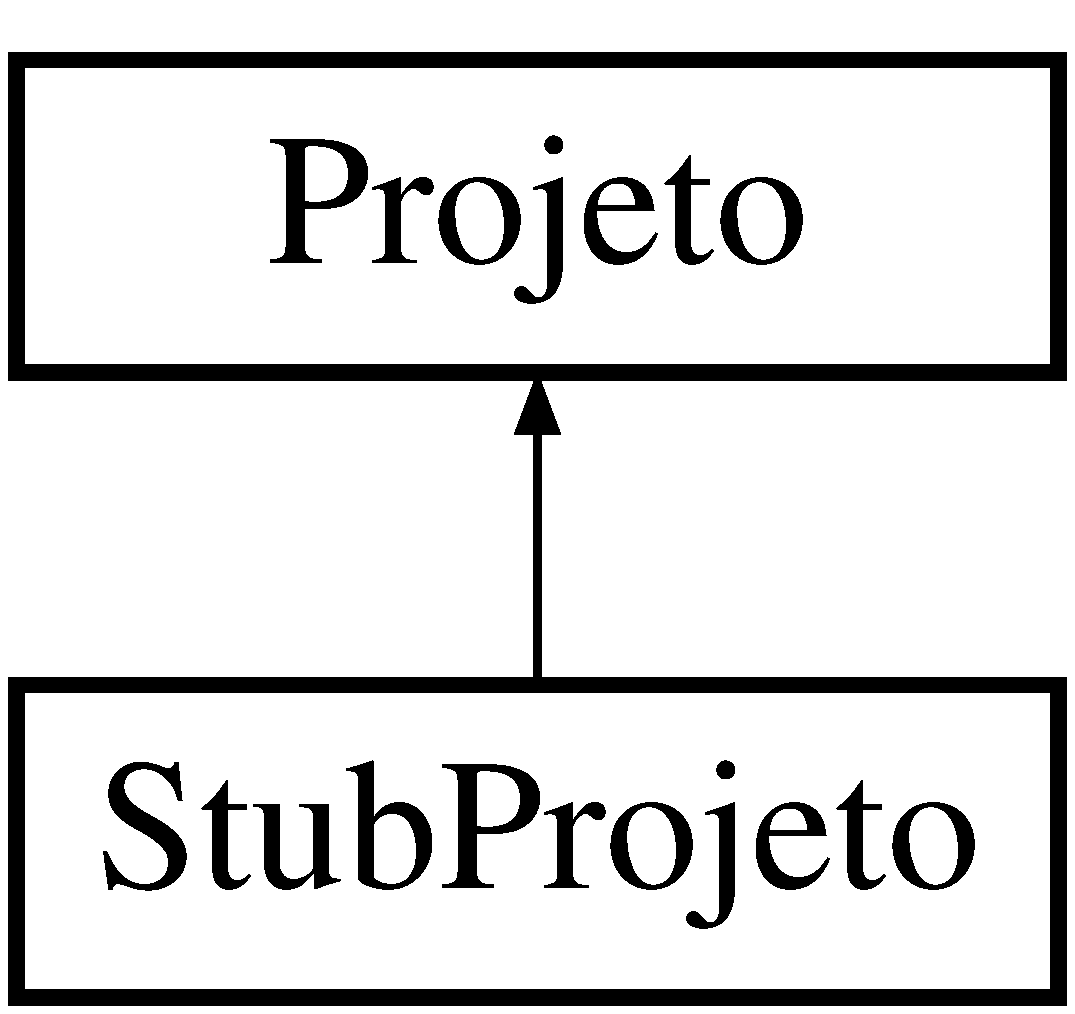
\includegraphics[height=2.000000cm]{class_projeto}
\end{center}
\end{figure}
\subsection*{\-Membros públicos}
\begin{DoxyCompactItemize}
\item 
\hypertarget{class_projeto_ab39919e206b2e33b6ab00bfa3bacd9a5}{
{\bfseries \-Projeto} (\hyperlink{class_matricula}{\-Matricula}, \hyperlink{class_codigo___projeto}{\-Codigo\-\_\-\-Projeto}, \hyperlink{class_data___inicio}{\-Data\-\_\-\-Inicio}, \hyperlink{class_data___termino}{\-Data\-\_\-\-Termino}, \hyperlink{class_nota}{\-Nota})}
\label{class_projeto_ab39919e206b2e33b6ab00bfa3bacd9a5}

\item 
\hyperlink{class_matricula}{\-Matricula} \hyperlink{class_projeto_ab5086bc8a75d77f2065639a836db28c9}{get\-Matricula} () const 
\begin{DoxyCompactList}\small\item\em \-Retorna o valor de \hyperlink{class_matricula}{\-Matricula} da entidade \hyperlink{class_projeto}{\-Projeto}. \end{DoxyCompactList}\item 
void \hyperlink{class_projeto_a2f220b68285d6acefe2b406520326969}{set\-Matricula} (const \hyperlink{class_matricula}{\-Matricula} \&)
\begin{DoxyCompactList}\small\item\em \-Seta o valor de \hyperlink{class_matricula}{\-Matricula} da entidade \hyperlink{class_projeto}{\-Projeto}. \end{DoxyCompactList}\item 
\hyperlink{class_codigo___projeto}{\-Codigo\-\_\-\-Projeto} \hyperlink{class_projeto_a1db1b38d1321c48894e74b7ac679b6e8}{get\-Codigo\-\_\-\-Projeto} () const 
\begin{DoxyCompactList}\small\item\em \-Retorna o valor de \-Codigo de \hyperlink{class_projeto}{\-Projeto} da entidade \hyperlink{class_projeto}{\-Projeto}. \end{DoxyCompactList}\item 
void \hyperlink{class_projeto_aba31c1e58bebad9aa88e4dfc41897bd5}{set\-Codigo\-\_\-\-Projeto} (const \hyperlink{class_codigo___projeto}{\-Codigo\-\_\-\-Projeto} \&)
\begin{DoxyCompactList}\small\item\em \-Seta o valor de \-Codigo de \hyperlink{class_projeto}{\-Projeto} da entidade \hyperlink{class_projeto}{\-Projeto}. \end{DoxyCompactList}\item 
\hyperlink{class_data___inicio}{\-Data\-\_\-\-Inicio} \hyperlink{class_projeto_a309461d7f136b25d6624b054c7beb3f0}{get\-Data\-\_\-\-Inicio} () const 
\begin{DoxyCompactList}\small\item\em \-Retorna o valor de \-Data de \-Inicio da entidade \hyperlink{class_projeto}{\-Projeto}. \end{DoxyCompactList}\item 
void \hyperlink{class_projeto_a699ba726969093cf54a3b1a7677c4434}{set\-Data\-\_\-\-Inicio} (const \hyperlink{class_data___inicio}{\-Data\-\_\-\-Inicio} \&)
\begin{DoxyCompactList}\small\item\em \-Seta o valor de \-Data de \-Inicio da entidade \hyperlink{class_projeto}{\-Projeto}. \end{DoxyCompactList}\item 
\hyperlink{class_data___termino}{\-Data\-\_\-\-Termino} \hyperlink{class_projeto_ae29e37b6730fc277a460d864238df94b}{get\-Data\-\_\-\-Termino} () const 
\begin{DoxyCompactList}\small\item\em \-Retorna o valor de \-Data de \-Termino da entidade \hyperlink{class_projeto}{\-Projeto}. \end{DoxyCompactList}\item 
void \hyperlink{class_projeto_a5371af0d47b30cb46fcd02a4d5fde73f}{set\-Data\-\_\-\-Termino} (const \hyperlink{class_data___termino}{\-Data\-\_\-\-Termino} \&)
\begin{DoxyCompactList}\small\item\em \-Seta o valor de \-Data de \-Termino da entidade \hyperlink{class_projeto}{\-Projeto}. \end{DoxyCompactList}\item 
\hyperlink{class_nota}{\-Nota} \hyperlink{class_projeto_add8f77d42d9c5656456b7625f00c2c02}{get\-Nota} () const 
\begin{DoxyCompactList}\small\item\em \-Retorna o valor de \hyperlink{class_nota}{\-Nota} da entidade \hyperlink{class_projeto}{\-Projeto}. \end{DoxyCompactList}\item 
void \hyperlink{class_projeto_ad074101c3df39dea6c3569c75593f338}{set\-Nota} (const \hyperlink{class_nota}{\-Nota} \&)
\begin{DoxyCompactList}\small\item\em \-Seta o valor de \hyperlink{class_nota}{\-Nota} da entidade \hyperlink{class_projeto}{\-Projeto}. \end{DoxyCompactList}\end{DoxyCompactItemize}


\subsection{\-Descrição detalhada}
\-Classe que representa a entidade \hyperlink{class_projeto}{\-Projeto}. 

\-Contem os atributos que sao instancias das classes \hyperlink{class_matricula}{\-Matricula}, \hyperlink{class_codigo___projeto}{\-Codigo\-\_\-\-Projeto}, \hyperlink{class_data___inicio}{\-Data\-\_\-\-Inicio}, \hyperlink{class_data___termino}{\-Data\-\_\-\-Termino} e \hyperlink{class_nota}{\-Nota} 

\subsection{\-Documentação dos métodos}
\hypertarget{class_projeto_a1db1b38d1321c48894e74b7ac679b6e8}{
\index{\-Projeto@{\-Projeto}!get\-Codigo\-\_\-\-Projeto@{get\-Codigo\-\_\-\-Projeto}}
\index{get\-Codigo\-\_\-\-Projeto@{get\-Codigo\-\_\-\-Projeto}!Projeto@{\-Projeto}}
\subsubsection[{get\-Codigo\-\_\-\-Projeto}]{\setlength{\rightskip}{0pt plus 5cm}{\bf \-Codigo\-\_\-\-Projeto} \-Projeto\-::get\-Codigo\-\_\-\-Projeto (
\begin{DoxyParamCaption}
{}
\end{DoxyParamCaption}
) const\hspace{0.3cm}{\ttfamily  \mbox{[}inline\mbox{]}}}}
\label{class_projeto_a1db1b38d1321c48894e74b7ac679b6e8}


\-Retorna o valor de \-Codigo de \hyperlink{class_projeto}{\-Projeto} da entidade \hyperlink{class_projeto}{\-Projeto}. 

\begin{DoxyReturn}{\-Retorna}
codigo\-\_\-projeto 
\end{DoxyReturn}
\hypertarget{class_projeto_a309461d7f136b25d6624b054c7beb3f0}{
\index{\-Projeto@{\-Projeto}!get\-Data\-\_\-\-Inicio@{get\-Data\-\_\-\-Inicio}}
\index{get\-Data\-\_\-\-Inicio@{get\-Data\-\_\-\-Inicio}!Projeto@{\-Projeto}}
\subsubsection[{get\-Data\-\_\-\-Inicio}]{\setlength{\rightskip}{0pt plus 5cm}{\bf \-Data\-\_\-\-Inicio} \-Projeto\-::get\-Data\-\_\-\-Inicio (
\begin{DoxyParamCaption}
{}
\end{DoxyParamCaption}
) const\hspace{0.3cm}{\ttfamily  \mbox{[}inline\mbox{]}}}}
\label{class_projeto_a309461d7f136b25d6624b054c7beb3f0}


\-Retorna o valor de \-Data de \-Inicio da entidade \hyperlink{class_projeto}{\-Projeto}. 

\begin{DoxyReturn}{\-Retorna}
data\-\_\-inicio 
\end{DoxyReturn}
\hypertarget{class_projeto_ae29e37b6730fc277a460d864238df94b}{
\index{\-Projeto@{\-Projeto}!get\-Data\-\_\-\-Termino@{get\-Data\-\_\-\-Termino}}
\index{get\-Data\-\_\-\-Termino@{get\-Data\-\_\-\-Termino}!Projeto@{\-Projeto}}
\subsubsection[{get\-Data\-\_\-\-Termino}]{\setlength{\rightskip}{0pt plus 5cm}{\bf \-Data\-\_\-\-Termino} \-Projeto\-::get\-Data\-\_\-\-Termino (
\begin{DoxyParamCaption}
{}
\end{DoxyParamCaption}
) const\hspace{0.3cm}{\ttfamily  \mbox{[}inline\mbox{]}}}}
\label{class_projeto_ae29e37b6730fc277a460d864238df94b}


\-Retorna o valor de \-Data de \-Termino da entidade \hyperlink{class_projeto}{\-Projeto}. 

\begin{DoxyReturn}{\-Retorna}
data\-\_\-termino 
\end{DoxyReturn}
\hypertarget{class_projeto_ab5086bc8a75d77f2065639a836db28c9}{
\index{\-Projeto@{\-Projeto}!get\-Matricula@{get\-Matricula}}
\index{get\-Matricula@{get\-Matricula}!Projeto@{\-Projeto}}
\subsubsection[{get\-Matricula}]{\setlength{\rightskip}{0pt plus 5cm}{\bf \-Matricula} \-Projeto\-::get\-Matricula (
\begin{DoxyParamCaption}
{}
\end{DoxyParamCaption}
) const\hspace{0.3cm}{\ttfamily  \mbox{[}inline\mbox{]}}}}
\label{class_projeto_ab5086bc8a75d77f2065639a836db28c9}


\-Retorna o valor de \hyperlink{class_matricula}{\-Matricula} da entidade \hyperlink{class_projeto}{\-Projeto}. 

\begin{DoxyReturn}{\-Retorna}
matricula 
\end{DoxyReturn}
\hypertarget{class_projeto_add8f77d42d9c5656456b7625f00c2c02}{
\index{\-Projeto@{\-Projeto}!get\-Nota@{get\-Nota}}
\index{get\-Nota@{get\-Nota}!Projeto@{\-Projeto}}
\subsubsection[{get\-Nota}]{\setlength{\rightskip}{0pt plus 5cm}{\bf \-Nota} \-Projeto\-::get\-Nota (
\begin{DoxyParamCaption}
{}
\end{DoxyParamCaption}
) const\hspace{0.3cm}{\ttfamily  \mbox{[}inline\mbox{]}}}}
\label{class_projeto_add8f77d42d9c5656456b7625f00c2c02}


\-Retorna o valor de \hyperlink{class_nota}{\-Nota} da entidade \hyperlink{class_projeto}{\-Projeto}. 

\begin{DoxyReturn}{\-Retorna}
nota 
\end{DoxyReturn}
\hypertarget{class_projeto_aba31c1e58bebad9aa88e4dfc41897bd5}{
\index{\-Projeto@{\-Projeto}!set\-Codigo\-\_\-\-Projeto@{set\-Codigo\-\_\-\-Projeto}}
\index{set\-Codigo\-\_\-\-Projeto@{set\-Codigo\-\_\-\-Projeto}!Projeto@{\-Projeto}}
\subsubsection[{set\-Codigo\-\_\-\-Projeto}]{\setlength{\rightskip}{0pt plus 5cm}void \-Projeto\-::set\-Codigo\-\_\-\-Projeto (
\begin{DoxyParamCaption}
\item[{const {\bf \-Codigo\-\_\-\-Projeto} \&}]{}
\end{DoxyParamCaption}
)}}
\label{class_projeto_aba31c1e58bebad9aa88e4dfc41897bd5}


\-Seta o valor de \-Codigo de \hyperlink{class_projeto}{\-Projeto} da entidade \hyperlink{class_projeto}{\-Projeto}. 


\begin{DoxyParams}{\-Parâmetros}
{\em \-Codigo\-\_\-\-Projeto\&} & \\
\hline
\end{DoxyParams}
\hypertarget{class_projeto_a699ba726969093cf54a3b1a7677c4434}{
\index{\-Projeto@{\-Projeto}!set\-Data\-\_\-\-Inicio@{set\-Data\-\_\-\-Inicio}}
\index{set\-Data\-\_\-\-Inicio@{set\-Data\-\_\-\-Inicio}!Projeto@{\-Projeto}}
\subsubsection[{set\-Data\-\_\-\-Inicio}]{\setlength{\rightskip}{0pt plus 5cm}void \-Projeto\-::set\-Data\-\_\-\-Inicio (
\begin{DoxyParamCaption}
\item[{const {\bf \-Data\-\_\-\-Inicio} \&}]{}
\end{DoxyParamCaption}
)}}
\label{class_projeto_a699ba726969093cf54a3b1a7677c4434}


\-Seta o valor de \-Data de \-Inicio da entidade \hyperlink{class_projeto}{\-Projeto}. 


\begin{DoxyParams}{\-Parâmetros}
{\em \-Data\-\_\-\-Inicio\&} & \\
\hline
\end{DoxyParams}
\hypertarget{class_projeto_a5371af0d47b30cb46fcd02a4d5fde73f}{
\index{\-Projeto@{\-Projeto}!set\-Data\-\_\-\-Termino@{set\-Data\-\_\-\-Termino}}
\index{set\-Data\-\_\-\-Termino@{set\-Data\-\_\-\-Termino}!Projeto@{\-Projeto}}
\subsubsection[{set\-Data\-\_\-\-Termino}]{\setlength{\rightskip}{0pt plus 5cm}void \-Projeto\-::set\-Data\-\_\-\-Termino (
\begin{DoxyParamCaption}
\item[{const {\bf \-Data\-\_\-\-Termino} \&}]{}
\end{DoxyParamCaption}
)}}
\label{class_projeto_a5371af0d47b30cb46fcd02a4d5fde73f}


\-Seta o valor de \-Data de \-Termino da entidade \hyperlink{class_projeto}{\-Projeto}. 


\begin{DoxyParams}{\-Parâmetros}
{\em \-Data\-\_\-\-Termino\&} & \\
\hline
\end{DoxyParams}
\hypertarget{class_projeto_a2f220b68285d6acefe2b406520326969}{
\index{\-Projeto@{\-Projeto}!set\-Matricula@{set\-Matricula}}
\index{set\-Matricula@{set\-Matricula}!Projeto@{\-Projeto}}
\subsubsection[{set\-Matricula}]{\setlength{\rightskip}{0pt plus 5cm}void \-Projeto\-::set\-Matricula (
\begin{DoxyParamCaption}
\item[{const {\bf \-Matricula} \&}]{}
\end{DoxyParamCaption}
)}}
\label{class_projeto_a2f220b68285d6acefe2b406520326969}


\-Seta o valor de \hyperlink{class_matricula}{\-Matricula} da entidade \hyperlink{class_projeto}{\-Projeto}. 


\begin{DoxyParams}{\-Parâmetros}
{\em \-Matricula\&} & \\
\hline
\end{DoxyParams}
\hypertarget{class_projeto_ad074101c3df39dea6c3569c75593f338}{
\index{\-Projeto@{\-Projeto}!set\-Nota@{set\-Nota}}
\index{set\-Nota@{set\-Nota}!Projeto@{\-Projeto}}
\subsubsection[{set\-Nota}]{\setlength{\rightskip}{0pt plus 5cm}void \-Projeto\-::set\-Nota (
\begin{DoxyParamCaption}
\item[{const {\bf \-Nota} \&}]{}
\end{DoxyParamCaption}
)}}
\label{class_projeto_ad074101c3df39dea6c3569c75593f338}


\-Seta o valor de \hyperlink{class_nota}{\-Nota} da entidade \hyperlink{class_projeto}{\-Projeto}. 


\begin{DoxyParams}{\-Parâmetros}
{\em \-Nota\&} & \\
\hline
\end{DoxyParams}


\-A documentação para esta classe foi gerada a partir do seguinte ficheiro\-:\begin{DoxyCompactItemize}
\item 
\-Entidades.\-h\end{DoxyCompactItemize}

\hypertarget{class_tamanho}{
\section{\-Referência da \-Classe \-Tamanho}
\label{class_tamanho}\index{\-Tamanho@{\-Tamanho}}
}


\-Classe que representa o dominio \hyperlink{class_tamanho}{\-Tamanho}.  




{\ttfamily \#include $<$\-Dominios.\-h$>$}

\subsection*{\-Métodos \-Públicos}
\begin{DoxyCompactItemize}
\item 
\hypertarget{class_tamanho_a63541f3ebe1209729030e17b6a21236c}{
{\bfseries \-Tamanho} (unsigned int)  throw (invalid\-\_\-argument)}
\label{class_tamanho_a63541f3ebe1209729030e17b6a21236c}

\item 
void \hyperlink{class_tamanho_afb80c548279d5baa4f0ef163f7f564d0}{set\-Valor} (const unsigned int \&)  throw (invalid\-\_\-argument)
\begin{DoxyCompactList}\small\item\em \-Seta o valor de \hyperlink{class_tamanho}{\-Tamanho}. \end{DoxyCompactList}\item 
unsigned int \hyperlink{class_tamanho_a0150e086c4b3d37b9d98e34c34532a10}{get\-Valor} () const 
\begin{DoxyCompactList}\small\item\em \-Retorna o valor de \hyperlink{class_tamanho}{\-Tamanho}. \end{DoxyCompactList}\end{DoxyCompactItemize}


\subsection{\-Descrição \-Detalhada}
\-Classe que representa o dominio \hyperlink{class_tamanho}{\-Tamanho}. 

\-Armazena os atributos de \hyperlink{class_tamanho}{\-Tamanho} \-Em \-Linhas \-De \-Codigo apos validacao\-: valor de 0 a 1000 

\subsection{\-Métodos}
\hypertarget{class_tamanho_a0150e086c4b3d37b9d98e34c34532a10}{
\index{\-Tamanho@{\-Tamanho}!get\-Valor@{get\-Valor}}
\index{get\-Valor@{get\-Valor}!Tamanho@{\-Tamanho}}
\subsubsection[{get\-Valor}]{\setlength{\rightskip}{0pt plus 5cm}unsigned int \-Tamanho\-::get\-Valor (
\begin{DoxyParamCaption}
{}
\end{DoxyParamCaption}
) const\hspace{0.3cm}{\ttfamily  \mbox{[}inline\mbox{]}}}}
\label{class_tamanho_a0150e086c4b3d37b9d98e34c34532a10}


\-Retorna o valor de \hyperlink{class_tamanho}{\-Tamanho}. 

\begin{DoxyReturn}{\-Retorna}
valor 
\end{DoxyReturn}
\hypertarget{class_tamanho_afb80c548279d5baa4f0ef163f7f564d0}{
\index{\-Tamanho@{\-Tamanho}!set\-Valor@{set\-Valor}}
\index{set\-Valor@{set\-Valor}!Tamanho@{\-Tamanho}}
\subsubsection[{set\-Valor}]{\setlength{\rightskip}{0pt plus 5cm}void \-Tamanho\-::set\-Valor (
\begin{DoxyParamCaption}
\item[{const unsigned int \&}]{valor}
\end{DoxyParamCaption}
)  throw (invalid\-\_\-argument)\hspace{0.3cm}{\ttfamily  \mbox{[}inline\mbox{]}}}}
\label{class_tamanho_afb80c548279d5baa4f0ef163f7f564d0}


\-Seta o valor de \hyperlink{class_tamanho}{\-Tamanho}. 


\begin{DoxyParams}{\-Parâmetros}
{\em valor} & \\
\hline
\end{DoxyParams}


\-A documentação para esta classe foi gerada a partir do seguinte arquivo\-:\begin{DoxyCompactItemize}
\item 
header/\-Dominios.\-h\end{DoxyCompactItemize}

\hypertarget{class_tempo}{
\section{\-Referência à classe \-Tempo}
\label{class_tempo}\index{\-Tempo@{\-Tempo}}
}


\-Classe que representa o dominio \hyperlink{class_tempo}{\-Tempo}.  




{\ttfamily \#include $<$\-Dominios.\-h$>$}

\subsection*{\-Membros públicos}
\begin{DoxyCompactItemize}
\item 
\hypertarget{class_tempo_adaa477ff29f28230aac7f70c32ac792b}{
{\bfseries \-Tempo} (string)  throw (invalid\-\_\-argument)}
\label{class_tempo_adaa477ff29f28230aac7f70c32ac792b}

\item 
void \hyperlink{class_tempo_aa692776272a35f0457c3610fbca8853e}{set\-Valor} (const string \&)  throw (invalid\-\_\-argument)
\begin{DoxyCompactList}\small\item\em \-Seta o valor de \hyperlink{class_tempo}{\-Tempo}. \end{DoxyCompactList}\item 
string \hyperlink{class_tempo_a52d19fafeba9848f5127906e0308c0b9}{get\-Valor} () const 
\begin{DoxyCompactList}\small\item\em \-Retorna o valor de \hyperlink{class_tamanho}{\-Tamanho}. \end{DoxyCompactList}\end{DoxyCompactItemize}


\subsection{\-Descrição detalhada}
\-Classe que representa o dominio \hyperlink{class_tempo}{\-Tempo}. 

\-Armazena os atributos de \hyperlink{class_tempo}{\-Tempo} apos validacao\-: valor de 0 a 2000 

\subsection{\-Documentação dos métodos}
\hypertarget{class_tempo_a52d19fafeba9848f5127906e0308c0b9}{
\index{\-Tempo@{\-Tempo}!get\-Valor@{get\-Valor}}
\index{get\-Valor@{get\-Valor}!Tempo@{\-Tempo}}
\subsubsection[{get\-Valor}]{\setlength{\rightskip}{0pt plus 5cm}string \-Tempo\-::get\-Valor (
\begin{DoxyParamCaption}
{}
\end{DoxyParamCaption}
) const\hspace{0.3cm}{\ttfamily  \mbox{[}inline\mbox{]}}}}
\label{class_tempo_a52d19fafeba9848f5127906e0308c0b9}


\-Retorna o valor de \hyperlink{class_tamanho}{\-Tamanho}. 

\begin{DoxyReturn}{\-Retorna}
valor 
\end{DoxyReturn}
\hypertarget{class_tempo_aa692776272a35f0457c3610fbca8853e}{
\index{\-Tempo@{\-Tempo}!set\-Valor@{set\-Valor}}
\index{set\-Valor@{set\-Valor}!Tempo@{\-Tempo}}
\subsubsection[{set\-Valor}]{\setlength{\rightskip}{0pt plus 5cm}void \-Tempo\-::set\-Valor (
\begin{DoxyParamCaption}
\item[{const string \&}]{valor}
\end{DoxyParamCaption}
)  throw (invalid\-\_\-argument)\hspace{0.3cm}{\ttfamily  \mbox{[}inline\mbox{]}}}}
\label{class_tempo_aa692776272a35f0457c3610fbca8853e}


\-Seta o valor de \hyperlink{class_tempo}{\-Tempo}. 


\begin{DoxyParams}{\-Parâmetros}
{\em valor} & \\
\hline
\end{DoxyParams}


\-A documentação para esta classe foi gerada a partir do seguinte ficheiro\-:\begin{DoxyCompactItemize}
\item 
\-Dominios.\-h\end{DoxyCompactItemize}

\printindex
\end{document}
